\documentclass{article}
\usepackage{amsmath, amssymb, ctex, graphicx, color}
\usepackage[margin=1in]{geometry}
\usepackage{setspace} % 行距控制
\usepackage{array}
\usepackage{makecell}
\usepackage{booktabs}

\usepackage{algorithm}
\usepackage{algpseudocode}
\usepackage{xcolor}
% 把默认注释符号 ▷ 改成行尾 // 等宽紫色，并右对齐
\renewcommand{\algorithmiccomment}[1]{\hfill\texttt{\textcolor{violet}{// #1}}}
% 定义 Input / Output 关键字（默认是 Require / Ensure）
\algnewcommand\algorithmicinput{\textbf{Input:}}
\algnewcommand\algorithmicoutput{\textbf{Output:}}
\algnewcommand\Input{\item[\algorithmicinput]}
\algnewcommand\Output{\item[\algorithmicoutput]}

\usepackage{titling}\setlength{\droptitle}{-2cm} 
\title{Ch8. Backpropagation \hfill 第8章 反向传播 \\ 
Section 8.1. Evaluation of Gradients \hfill 第8.1节 梯度计算 \\ 
8.1.1. Single-layer networks \hfill 8.1.1. 单层网络 \\
8.1.2. General feed-forward networks \hfill 8.1.2. 一般前馈网络}
\author{《深度学习基础》课程小组}
% \date{}
 
\begin{document}
\maketitle
% \tableofcontents

\setlength{\parindent}{0pt} % 取消首行缩进
\setlength{\parskip}{1.5em} % 设置段落之间的距离

\noindent\rule{\linewidth}{0.4pt}

\section{P1}

Our goal in this chapter is to find an efficient technique for evaluating the gradient of an error function $E(\mathbf{w})$ for a feed-forward neural network. We will see that this can be achieved using a local message-passing scheme in which information is sent backwards through the network and is known as \textit{error backpropagation}, or sometimes simply as \textit{backprop}.

\noindent\rule{\linewidth}{0.4pt}

\section{P2}

Historically, the backpropagation equations have been derived by hand and then implemented in software alongside the forward propagation equations, with both steps taking time and being prone to mistakes. Modern neural network software environments, however, allow virtually any derivatives of interest to be calculated efficiently with only minimal effort beyond that of coding up the original network function. This idea, called automatic differentiation, plays a key role in modern deep learning. However, it is valuable to understand how the calculations are performed so that we are not relying on ``black box'' software solutions. In this chapter we therefore explain the key concepts of backpropagation, and explore the framework of automatic differentiation in detail.

\noindent\rule{\linewidth}{0.4pt}

\section{P3}

Note that the term ``backpropagation'' is used in the neural computing literature in a variety of different ways. For instance, a feed-forward architecture may be called a backpropagation network. Also the term `backpropagation' is sometimes used to describe the end-to-end training procedure for a neural network including the gradient descent parameter updates. In this book we will use `backpropagation' specifically to describe the computational procedure used in the numerical evaluation of derivatives such as the gradient of the error function with respect to the weights and biases of a network. This procedure can also be applied to the evaluation of other important derivatives such as the Jacobian and Hessian matrices.

% \subsection{8.1. Evaluation of Gradients}

\noindent\rule{\linewidth}{0.4pt}

\section{P4}

We now derive the backpropagation algorithm for a general network having arbitrary feed-forward topology, arbitrary differentiable nonlinear activation functions, and a broad class of error function. The resulting formulae will then be illustrated using a simple layered network structure having a single layer of sigmoidal hidden units together with a sum-of-squares error.

\noindent\rule{\linewidth}{0.4pt}

\section{P5}

Many error functions of practical interest, for instance those defined by maximum likelihood for a set of i.i.d.\ data, comprise a sum of terms, one for each data point in the training set so that
\begin{equation}
    E(\mathbf{w}) = \sum_{n=1}^N E_n(\mathbf{w}).
    \tag{8.1}
\end{equation}
Here we will consider the problem of evaluating $\nabla E_n(\mathbf{w})$ for one such term in the error function. This may be used directly for stochastic gradient descent, or the results could be accumulated over a set of training data points for batch or mini-batch methods.

\noindent\rule{\linewidth}{0.4pt}

\section{P6 8.1.1. Single-layer networks}

Consider first a simple linear model in which the outputs $y_k$ are linear combinations of the input variables $x_i$ so that
\begin{equation}
    y_k = \sum_i w_{ki} x_i
    \tag{8.2}
\end{equation}
together with a sum-of-squares error function that, for a particular input data point $n$, takes the form
\begin{equation}
    E_n = \frac{1}{2} \sum_k (y_{nk} - t_{nk})^2
    \tag{8.3}
\end{equation}
where $y_{nk} = y_k(\mathbf{x}_n, \mathbf{w})$, and $t_{nk}$ is the associated target value. The gradient of this error function with respect to a weight $w_{ji}$ is given by
\begin{equation}
    \frac{\partial E_n}{\partial w_{ji}} = (y_{nj} - t_{nj}) x_{ni}.
    \tag{8.4}
\end{equation}
This can be interpreted as a `local' computation involving the product of an `error signal' $y_{nj} - t_{nj}$ associated with the output end of the link $w_{ji}$ and the variable $x_{ni}$ associated with the input end of the link. In Section 5.4.3, we saw a similar formula arises with the logistic-sigmoid activation function together with the cross-entropy error function and similarly for the softmax activation function together with its matching multivariate cross-entropy error function. We will now see how this simple result extends to the more complex setting of multilayer feed-forward networks.

\noindent\rule{\linewidth}{0.4pt}

\section{P7 8.1.2. General feed-forward networks}

In general, a feed-forward network consists of a set of units each of which computes a weighted sum of its inputs:
\begin{equation}
    a_j = \sum_i w_{ji} z_i
    \tag{8.5}
\end{equation}
where $z_i$ is either the activation of another unit or an input unit that sends a connection to unit $j$, and $w_{ji}$ is the weight associated with that connection. Biases can be included in this sum by introducing an extra unit, or input, with activation fixed at $+1$, and so we do not need to deal with biases explicitly. The sum in (8.5), known as a pre-activation, is transformed by a nonlinear activation function $h(\cdot)$ to give the activation $z_j$ of unit $j$ in the form
\begin{equation}
    z_j = h(a_j).
    \tag{8.6}
\end{equation}
Note that one or more of the variables $z_i$ in the sum in (8.5) could be an input, and similarly, the unit $j$ in (8.6) could be an output.

\noindent\rule{\linewidth}{0.4pt}

\section{P8}

For each data point in the training set, we will suppose that we have supplied the corresponding input vector to the network and calculated the activations of all the hidden and output units in the network by successive application of (8.5) and (8.6). This process is called \textit{forward propagation} because it can be regarded as a forward flow of information through the network.

\noindent\rule{\linewidth}{0.4pt}

\section{P9}

Now consider the evaluation of the derivative of $E_n$ with respect to a weight $w_{ji}$. The outputs of the various units will depend on the particular input data point $n$. However, to keep the notation uncluttered, we will omit the subscript $n$ from the network variables. First note that $E_n$ depends on the weight $w_{ji}$ only via the summed input $a_j$ to unit $j$. We can therefore apply the chain rule for partial derivatives to give
\begin{equation}
    \frac{\partial E_n}{\partial w_{ji}} = \frac{\partial E_n}{\partial a_j} \frac{\partial a_j}{\partial w_{ji}}.
    \tag{8.7}
\end{equation}
We now introduce a useful notation:
\begin{equation}
    \delta_j \equiv \frac{\partial E_n}{\partial a_j}
    \tag{8.8}
\end{equation}
where the $\delta$'s are often referred to as errors for reasons we will see shortly. 

Using (8.5), we can write
\begin{equation}
    \frac{\partial a_j}{\partial w_{ji}} = z_i.
    \tag{8.9}
\end{equation}
Substituting (8.8) and (8.9) into (8.7), we then obtain
\begin{equation}
    \frac{\partial E_n}{\partial w_{ji}} = \delta_j z_i.
    \tag{8.10}
\end{equation}
Equation (8.10) tells us that the required derivative is obtained simply by multiplying the value of $\delta$ for the unit at the output end of the weight by the value of $z$ for the unit at the input end of the weight (where $z = 1$ for a bias). Note that this takes the same form as that found for the simple linear model in (8.4). Thus, to evaluate the derivatives, we need calculate only the value of $\delta_j$ for each hidden and output unit in the network and then apply (8.10).

\noindent\rule{\linewidth}{0.4pt}

\section{P10}

As we have seen already, for the output units, we have
\begin{equation}
    \delta_k = y_k - t_k
    \tag{8.11}
\end{equation}
provided we are using the canonical link as the output-unit activation function. To evaluate the $\delta$'s for hidden units, we again make use of the chain rule for partial derivatives:
\begin{equation}
    \delta_j \equiv \frac{\partial E_n}{\partial a_j} = \sum_k \frac{\partial E_n}{\partial a_k} \frac{\partial a_k}{\partial a_j}.
    \tag{8.12}
\end{equation}
where the sum runs over all units $k$ to which unit $j$ sends connections. The arrangement of units and weights is illustrated in Figure~\ref{fig:backprop_diagram}. Note that the units labelled $k$ include other hidden units and/or output units. In writing down (8.12), we are making use of the fact that variations in $a_j$ give rise to variations in the error function only through variations in the variables $a_k$.

Figure 8.1 Caption: Illustration of the calculation of $\delta_j$ for hidden unit $j$ by backpropagation of the $\delta$'s from those units $k$ to which unit $j$ sends connections. The black arrows denote the direction of information flow during forward propagation, and the red arrows indicate the backward propagation of error information.

\begin{figure}[htbp]
    \centering
    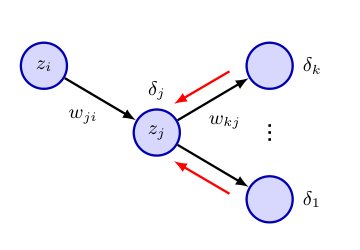
\includegraphics[width=0.5\textwidth]{figure-8-1.png}
    \caption{激活值（信息） $z$ 向右传播，误差 $\delta$ 向左传播}
    \label{fig:backprop_diagram}
\end{figure}

\noindent\rule{\linewidth}{0.4pt}

\section{P11}

If we now substitute the definition of $\delta_j$ given by (8.8) into (8.12) and make use of (8.5) and (8.6), we obtain the following backpropagation formula:
\begin{equation}
    \delta_j = h'(a_j) \sum_k w_{kj} \delta_k.
    \tag{8.13}
\end{equation}
which tells us that the value of $\delta$ for a particular hidden unit can be obtained by propagating the $\delta$'s backwards through the network, starting with those for the output units, whose values are already known. Note that the summation in (8.13) is taken over the first index on $w_{kj}$ (corresponding to backward propagation of information through the network), whereas in the forward propagation equation (8.5), it is taken over the second index. Because we already know the values of the $\delta$'s for the output units, it follows that by recursively applying (8.13), we can evaluate the $\delta$'s for all the hidden units in a feed-forward network, regardless of its topology. The backpropagation procedure is summarized in Algorithm~\ref{alg:backprop}.

\begin{algorithm}[H]
\caption{Backpropagation}
\label{alg:backprop}
\begin{algorithmic}[1]
\Require Input vector $\mathbf{x}_n$ \\
         Network parameters $\mathbf{w}$ \\
         Error function $E_n(\mathbf{w})$ for input $\mathbf{x}_n$ \\
         Activation function $h(a_j)$
\Ensure Error function derivatives $\{\partial E_n / \partial w_{ji}\}$
\State // Forward propagation
\For{$j \in$ all hidden and output units}
    \State $a_j \leftarrow \sum_i w_{ji} z_i$ \Comment{includes inputs $\{x_i\}$}
    \State $z_j \leftarrow h(a_j)$ \Comment{activation function}
\EndFor
\State // Error evaluation
\For{$k \in$ all output units}
    \State $\delta_k \leftarrow \frac{\partial E_n}{\partial a_k}$ \Comment{compute errors}
\EndFor
\State // Backward propagation, in reverse order
\For{$j \in$ all hidden units}
    \State $\delta_j \leftarrow h'(a_j) \sum_k w_{kj} \delta_k$ \Comment{recursive backward evaluation}
    \State $\frac{\partial E_n}{\partial w_{ji}} \leftarrow \delta_j z_i$ \Comment{evaluate derivatives}
\EndFor
\State \Return $\{\frac{\partial E_n}{\partial w_{ji}}\}$
\end{algorithmic}
\end{algorithm}

\noindent\rule{\linewidth}{0.4pt}

\section{P12}

For batch methods, the derivative of the total error $E$ can then be obtained by repeating the above steps for each data point in the training set and then summing over all data points in the batch or mini-batch.
\begin{equation}
    \frac{\partial E}{\partial w_{ji}} = \sum_n \frac{\partial E_n}{\partial w_{ji}}.
    \tag{8.14}
\end{equation}

\noindent\rule{\linewidth}{0.4pt}

\section{P13}

In the above derivation we have implicitly assumed that each hidden or output unit in the network has the same activation function $h(\cdot)$. However, the derivation is easily generalized to allow different units to have individual activation functions, simply by keeping track of which form of $h(\cdot)$ goes with which unit.

\end{document}
